\documentclass[11pt,a4]{article}
\usepackage[slovene]{babel}
\usepackage{natbib}
\usepackage{url}
\usepackage[utf8x]{inputenc}
\usepackage{amsmath,amssymb,latexsym}
\usepackage{graphicx}
\usepackage{parskip}
\usepackage{fancyhdr}
\usepackage{vmargin}
\setmarginsrb{3 cm}{2.5 cm}{3 cm}{2.5 cm}{1 cm}{1.5 cm}{1 cm}{1.5 cm}

% HyperRef
\usepackage[usenames,pdfnames]{xcolor}
\usepackage{hyperref}
\hypersetup{
	colorlinks = true,
	linkcolor = {red!50!black},
	citecolor = {blue!50!black},
	urlcolor = {blue!80!black}
}

% Title
\title{Teleskop kot pripomoček pri astronomski navigaciji}
\date{\today}
\author{}

\makeatletter
\let\thetitle\@title
\let\theauthor\@author
\let\thedate\@date
\makeatother

\pagestyle{fancy}
\fancyhf{}
\rhead{\theauthor}
\lhead{\thetitle}
\cfoot{\thepage}

\begin{document}

%%%%%%%%%%%%%%%%%%%%%%%%%%%%%%%%%%%%%%%%%%%%%%%%%%%%%%%%%%%%%%%%%%%%%%%%%%%%%%%%%%%%%%%%%

\begin{titlepage}
	\centering
	\vspace*{-2cm}
    
\includegraphics[scale = 0.75]{logo_FPP.png}\\[1.0 cm]
    
	\rule{\linewidth}{1 mm} \\[0.4 cm]
	{ \huge \bfseries Ladijske elektronske naprave} \\[0.5 cm]
	{ \Large \bfseries Navodila seminarske naloge}
	\rule{\linewidth}{1 mm} \\[1 cm]
	
	\rule{\linewidth}{0.5 mm} \\[0.4 cm]
	{ \large \bfseries \thetitle}\\[0.0 cm]
	\rule{\linewidth}{0.5 mm} \\[2 cm]
	
	\begin{minipage}{0.4\textwidth}
		\begin{flushleft} \large
			\emph{Avtorji:}\\[0.2 cm]
			Aleksander GRM\\
			Franc DIMC\\
			Darjan JAGNJIĆ
			\end{flushleft}
			\end{minipage}~
			\begin{minipage}{0.4\textwidth}
			\begin{flushright}
			\end{flushright}
	\end{minipage}\\[2 cm]
	
	\vfill
	
	{\large \thedate}\\[2 cm]
 
	
	
\end{titlepage}

%%%%%%%%%%%%%%%%%%%%%%%%%%%%%%%%%%%%%%%%%%%%%%%%%%%%%%%%%%%%%%%%%%%%%%%%%%%%%%%%%%%%%%%%%

\tableofcontents
\pagebreak

%%%%%%%%%%%%%%%%%%%%%%%%%%%%%%%%%%%%%%%%%%%%%%%%%%%%%%%%%%%%%%%%%%%%%%%%%%%%%%%%%%%%%%%%%

\section{Uvod}
Teleskopi so optični pripomočki, ki jih uporabljamo v astronomiji za opazovanje astronomskih objektov kot so planeti, zvezde, galaksije, kometi, itd. Za gledanje astronomskih objektov lahko uporabljamo optične ali elektronske pripomočke.

Z uporabo optičnega pripomočka ali okularja, gledamo astronomske objekte s prostim očesom. Okularjev je več, kjer je najbolj pomembna lastnost povečava okularja kar pomeni, da si lahko spreminjamo vidno polje. Vidno polje je povezano z velikostjo objekta, ki ga opazujemo, kot je recimo, planet, galaksija ali zvezda.

Z uporabo elektronske naprava ali senzorja pa nadomestimo naše oko z elektronskim senzorjem. V našem primeru je to CCD kamera. Kakor okularjev obstaja tudi več vrst kamer, ki se uporabljajo za različne namene. 
  
Zaradi svojega natančnega sledilnega mehanizma, lahko s teleskopom zelo natančno določimo višino in azimut astronomskega objekt. To sta dva najbolj pomembna merska podatka v astronomski navigaciji. Na ladji višino merimo s sekstantom, azimut pa s smerno napravo. V astronomski navigaciji se ponavadi uporabljajo najbolj svetle zvezde in planete. 

\begin{figure}[tb]
	\begin{center}
		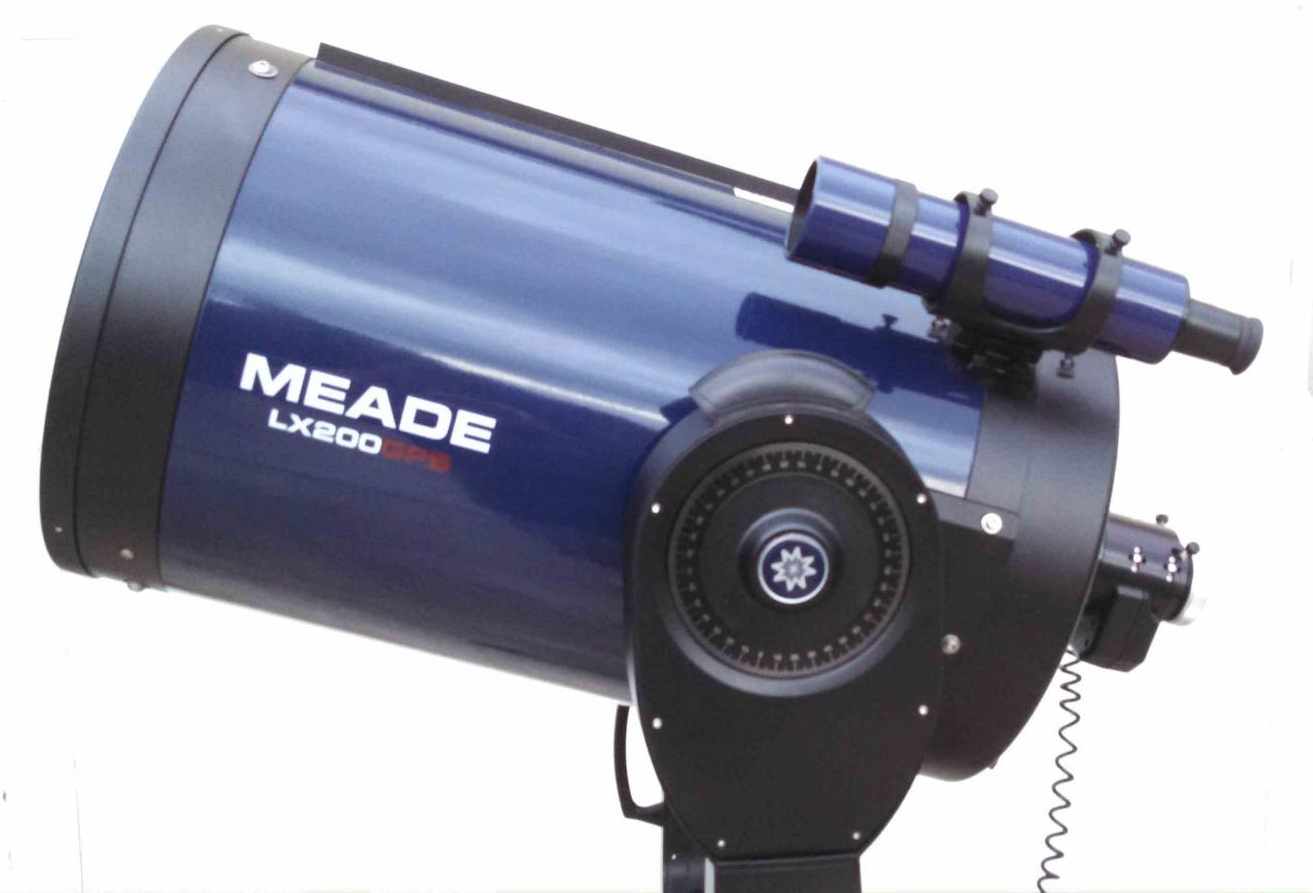
\includegraphics[width=12cm]{figs/meade_lx200gps.png}
	\end{center}
\caption{Šolski teleskop Meade LX200GPS. Premer zrcala 14 palcev.}
\end{figure}

\pagebreak

\section{Naloga}

V okviru zadane naloge se bomo naredili prve korake pri uporabi

\begin{itemize}
	\item Navtični almanah,
	\item Zvezdne karte,
	\item Zvezdni identifikator,
	\item Uporabiti teleskop za izmero višine in azimuta astronomskega objekta,
	\item Določanje astronomskega položaja s pomočjo izmerjenih podatkov,
\end{itemize}

ki jih boste lahko nato s pridom uporabili pri predmetu \textit{Oceanska navigacija}.

\subsection{Navtični almanah}
Navtični almanah vsebuje pomembne podatke o astronomskih objektih in koordinatnem sistemu. Kot primer, si lahko pregledate brezplačen dostop do navtičnih astronomskih podatkov na povezavi \href{https://thenauticalalmanac.com/}{thenauticalalmanac.com}. V navtičnem almanahu se nahajajo podatki, ki jih potrebujemo za identificiranje astronomskih objektov in kasneje določanje astronomskega položaja s pomočjo izmerjenih podatkov.

\subsection{Zvezdne karte}
S pomočjo zvezdnih kart lahko približno sledimo strukturi nebesnih teles na nebu. Zvezdni karti sta ponavadi dve in sicer za severno in južno astronomsko nebo. Na karti imamo narisane in označene večino astronomskih objektov. Mi bomo uporabili elektronske astronomske karte in sicer \href{http://www.stellarium.org/}{Stellarium}.

\subsection{Zvezdni identifikator} 
kot primer zvezdnega identifikatorja si bomo pogledali Kotlaričev zvezdni identifikator. S pomočjo navtičnega almanaha in identifikatorja, lahko izjemno enostavno določimo katero svetlo zvezdo opazujemo.

\subsection{Teleskop}
S pomočjo asistenta boste videli, kako se teleskop uporablja. S teleskopom bomo sledili določeni zvezdi ali planetu, videli boste tirnice gibanja in določili osnovne parametre, ko so deklinacija, rektascenzija, višina in azimut. S pomočjo izmerjenih podatkov boste nato lahko določili vaš astronomski položaj.

\subsection{Določanje astronomskega položaja}
Z izmerjenimi podatki in podatki iz navtičnega almanaha bomo določili položaj na dva načina. Prvi je grafičen z uporabo bele karte, na katero boste vrisali izračunane podatke. V drugem načinu bomo pa položaj določili čisto računsko s pomočjo izračunanih podatkov in presečišča krožnic. 

Veliko o metodah si lahko pogledate na \href{https://sites.google.com/site/navigationalalgorithms}{Navigational Algorithms}. Možnost je tudi učenje preko e-učilnice \href{https://my.vanderbilt.edu/astronav}{Astro Nav}.

\section{Izvedba naloge in zadolžitve študentov}
Naloga se izvede v več sklopih in sicer

\begin{itemize}
	\item predstavitev naloge, debata o vsebini in predvidenih rezultatih, določimo vire in roke za napredovanje in kontrolo,
	\item izvedemo teoretičen del naloge, kjer spoznamo navtični almanah, identifikator zvezd in metodo določanja astronomskega položaja,
	\item na ugodno noč se dobimo in naredimo uvodne meritve, vajo lahko ponovimo še en večer,
	\item študentje se dobijo, prevetrijo rezultate in pričnejo s pisanjem zaključnega poročila naloge,
	\item na koncu se poročilo odda in sledi zagovor naloge.  
\end{itemize}

\section*{Literatura}
\begin{itemize}
	\item \href{https://drive.google.com/open?id=0B1dT-CBA07ANZGNEUlc1MEtlZXM}{LEN seminar teleskop}
\end{itemize}

%\bibliographystyle{plain}
%\bibliography{literatura}

\end{document}